\chapter{System modelling}\label{chap:systemmodelling}
For the system modeling, the simplified physics to calculate lift and rotational velocity of the drone from section \ref{sec:preliminaryphysics} will be used. The model is implemented with Simscape Multibody, an add-on of Matlab Simulink.\\

The drone body was developed in Solidworks, seen in fig. \ref{fig:drone3D}. The PCBs, RPi, and battery pack have been assumed as an equal mass distribution on each arm of the drone. As such, they have not been implemented visually in the model.
\begin{figure}[h!]
    \centering
    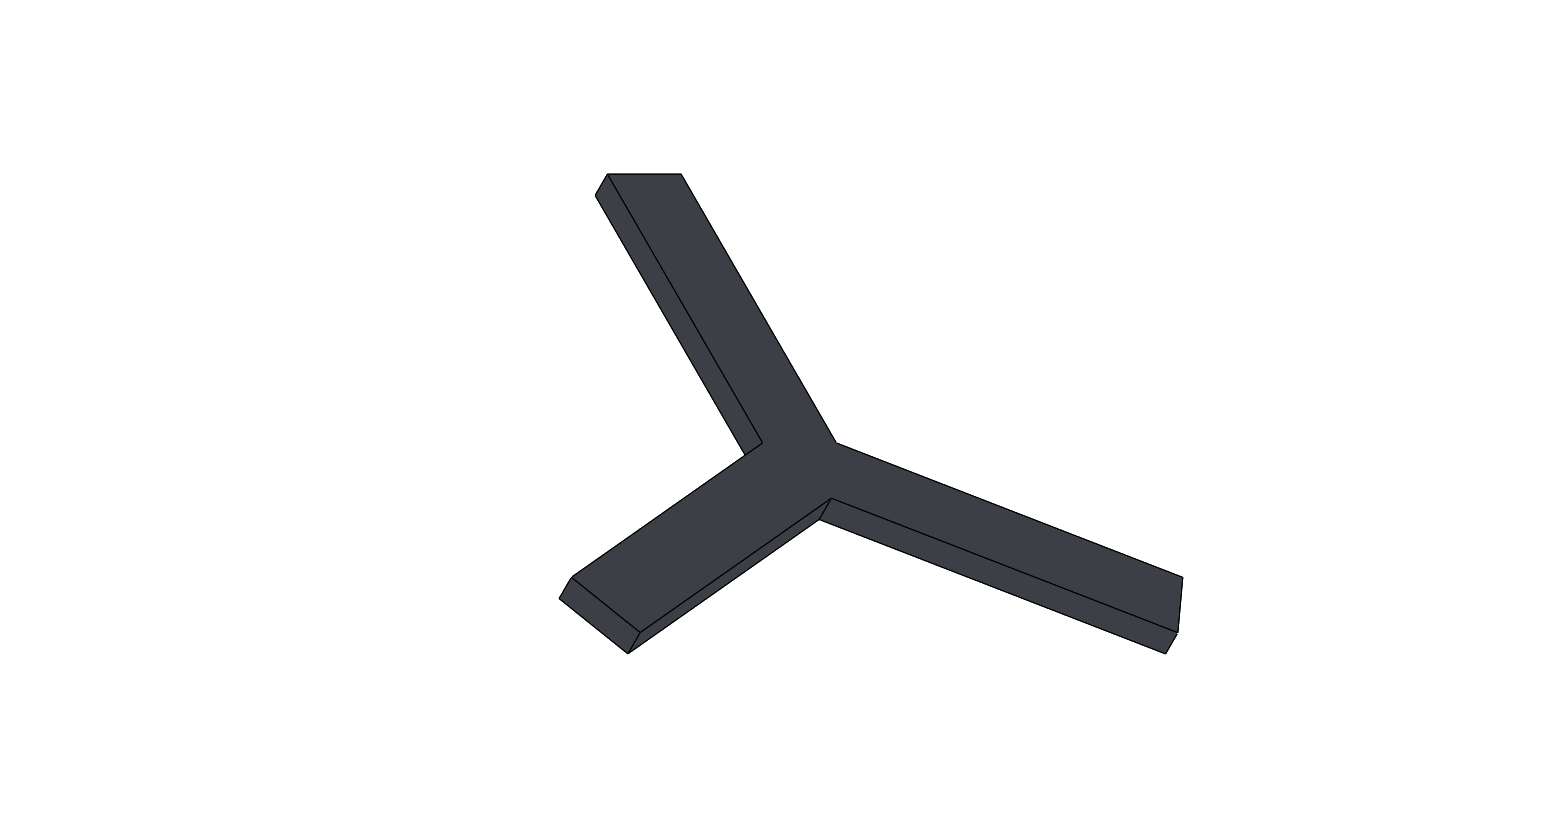
\includegraphics[width=0.7\textwidth]{figures/system_modelling/drone3d.PNG}
    \caption{3D model of the drone's body excluding wings and propeller motors -- constructed in Solidworks}
    \label{fig:drone3D}
\end{figure}
Subsequently, the motors and wings were added to the model to simulate the physical forces acting on the drone. The physics are also implemented using the equations of chapter \ref{sec:preliminaryphysics}. Although for the sake of computational simplicity, the lift is generated by eq. \ref{eq:model_lift}.\\
\begin{equation}
    \label{eq:model_lift}
    L = \frac{1}{2}*A_{wing}*c_L*\rho*\left(\omega*\left(r_{inner}+\frac{L_{wing}}{2}\right)\right)^2
\end{equation}
The wings' drag and lift coefficient are dynamic and thus implemented with a look-up table.\\

The final model is implemented with many subsystems that model different physical properties. The model consists of subsystems for: 
\begin{itemize}[noitemsep]
    \item Wing physics
    \item Motor physics
    \item Coordinate reference
    \item Controller blocks
    \item Measurement facilitation in all of the above
\end{itemize}

The final visual appearance of the modelled drone is shown in fig. \ref{fig:fullmodeldrone}.
\begin{figure}[h!]
    \centering
    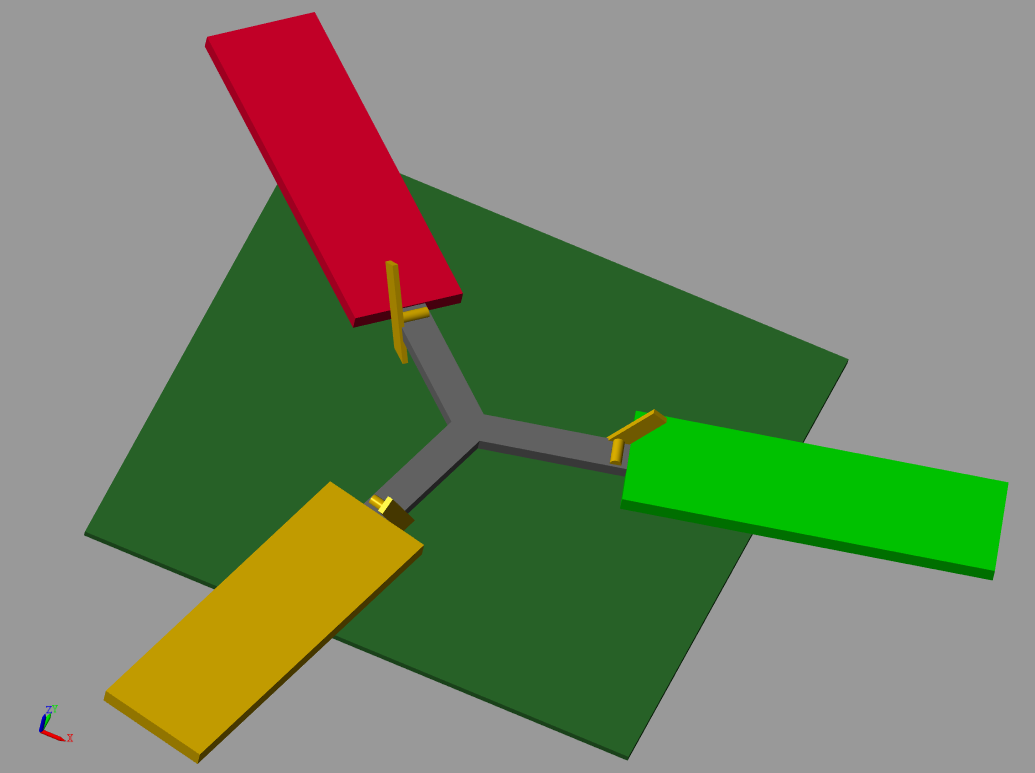
\includegraphics[width=0.5\textwidth]{figures/system_modelling/drone_full_physical_appearance.PNG}
    \caption{The drone model with wings and prop motors}
    \label{fig:fullmodeldrone}
\end{figure}

The top level of the Simulink model can be seen in fig. \ref{fig:toplevelmodel}.

\section{From reality to model and back}
The drag of both motors and wings will be adjusted so that the model fits the real drone's measured data while airborne. \\
The model's natural transfer function will be derived in the same way as with the drone. This is done by stepping the drone at a steady-state. \\

As a result, the model will be used to implement and adjust any proposed rotational controller quickly. Furthermore, it is agile and easy to adjust for changes to the system, or to include new controllers of i.e., height or tilt. The model files are attached to the hand-in.

\section{Chapter summary}
A model of the drone using simplified physics has been implemented using Simscape Multibody in Matlab. The objective outlined in section \ref{modelgoals} has been achieved. Deriving a transfer function and comparing the model with the actual drone will be done in section \ref{sec:modelresponse}. 